\section*{A-3. データ収集から特徴量抽出}
この章では,BLEを用いた混雑度推定手法について述べる.

\subsection*{3.1 BLEスキャンと正解ラベルの取得}
この章では,学生食堂内のBLEデータと,その時点の食堂利用人数の計測方法を述べる.

\subsubsection*{Raspberry PiによるBLEスキャン}
BLEスキャンは図\ref{raspi}のようなRaspberry Piを用いて行う.
スキャンは約10秒の間隔で行われ,1回のスキャンに含まれる情報は以下の通りである.
\begin{itemize}
  \item BLE情報(MACアドレス,RSSI)
  \item スキャン時刻
\end{itemize}

\begin{figure}[pt]
  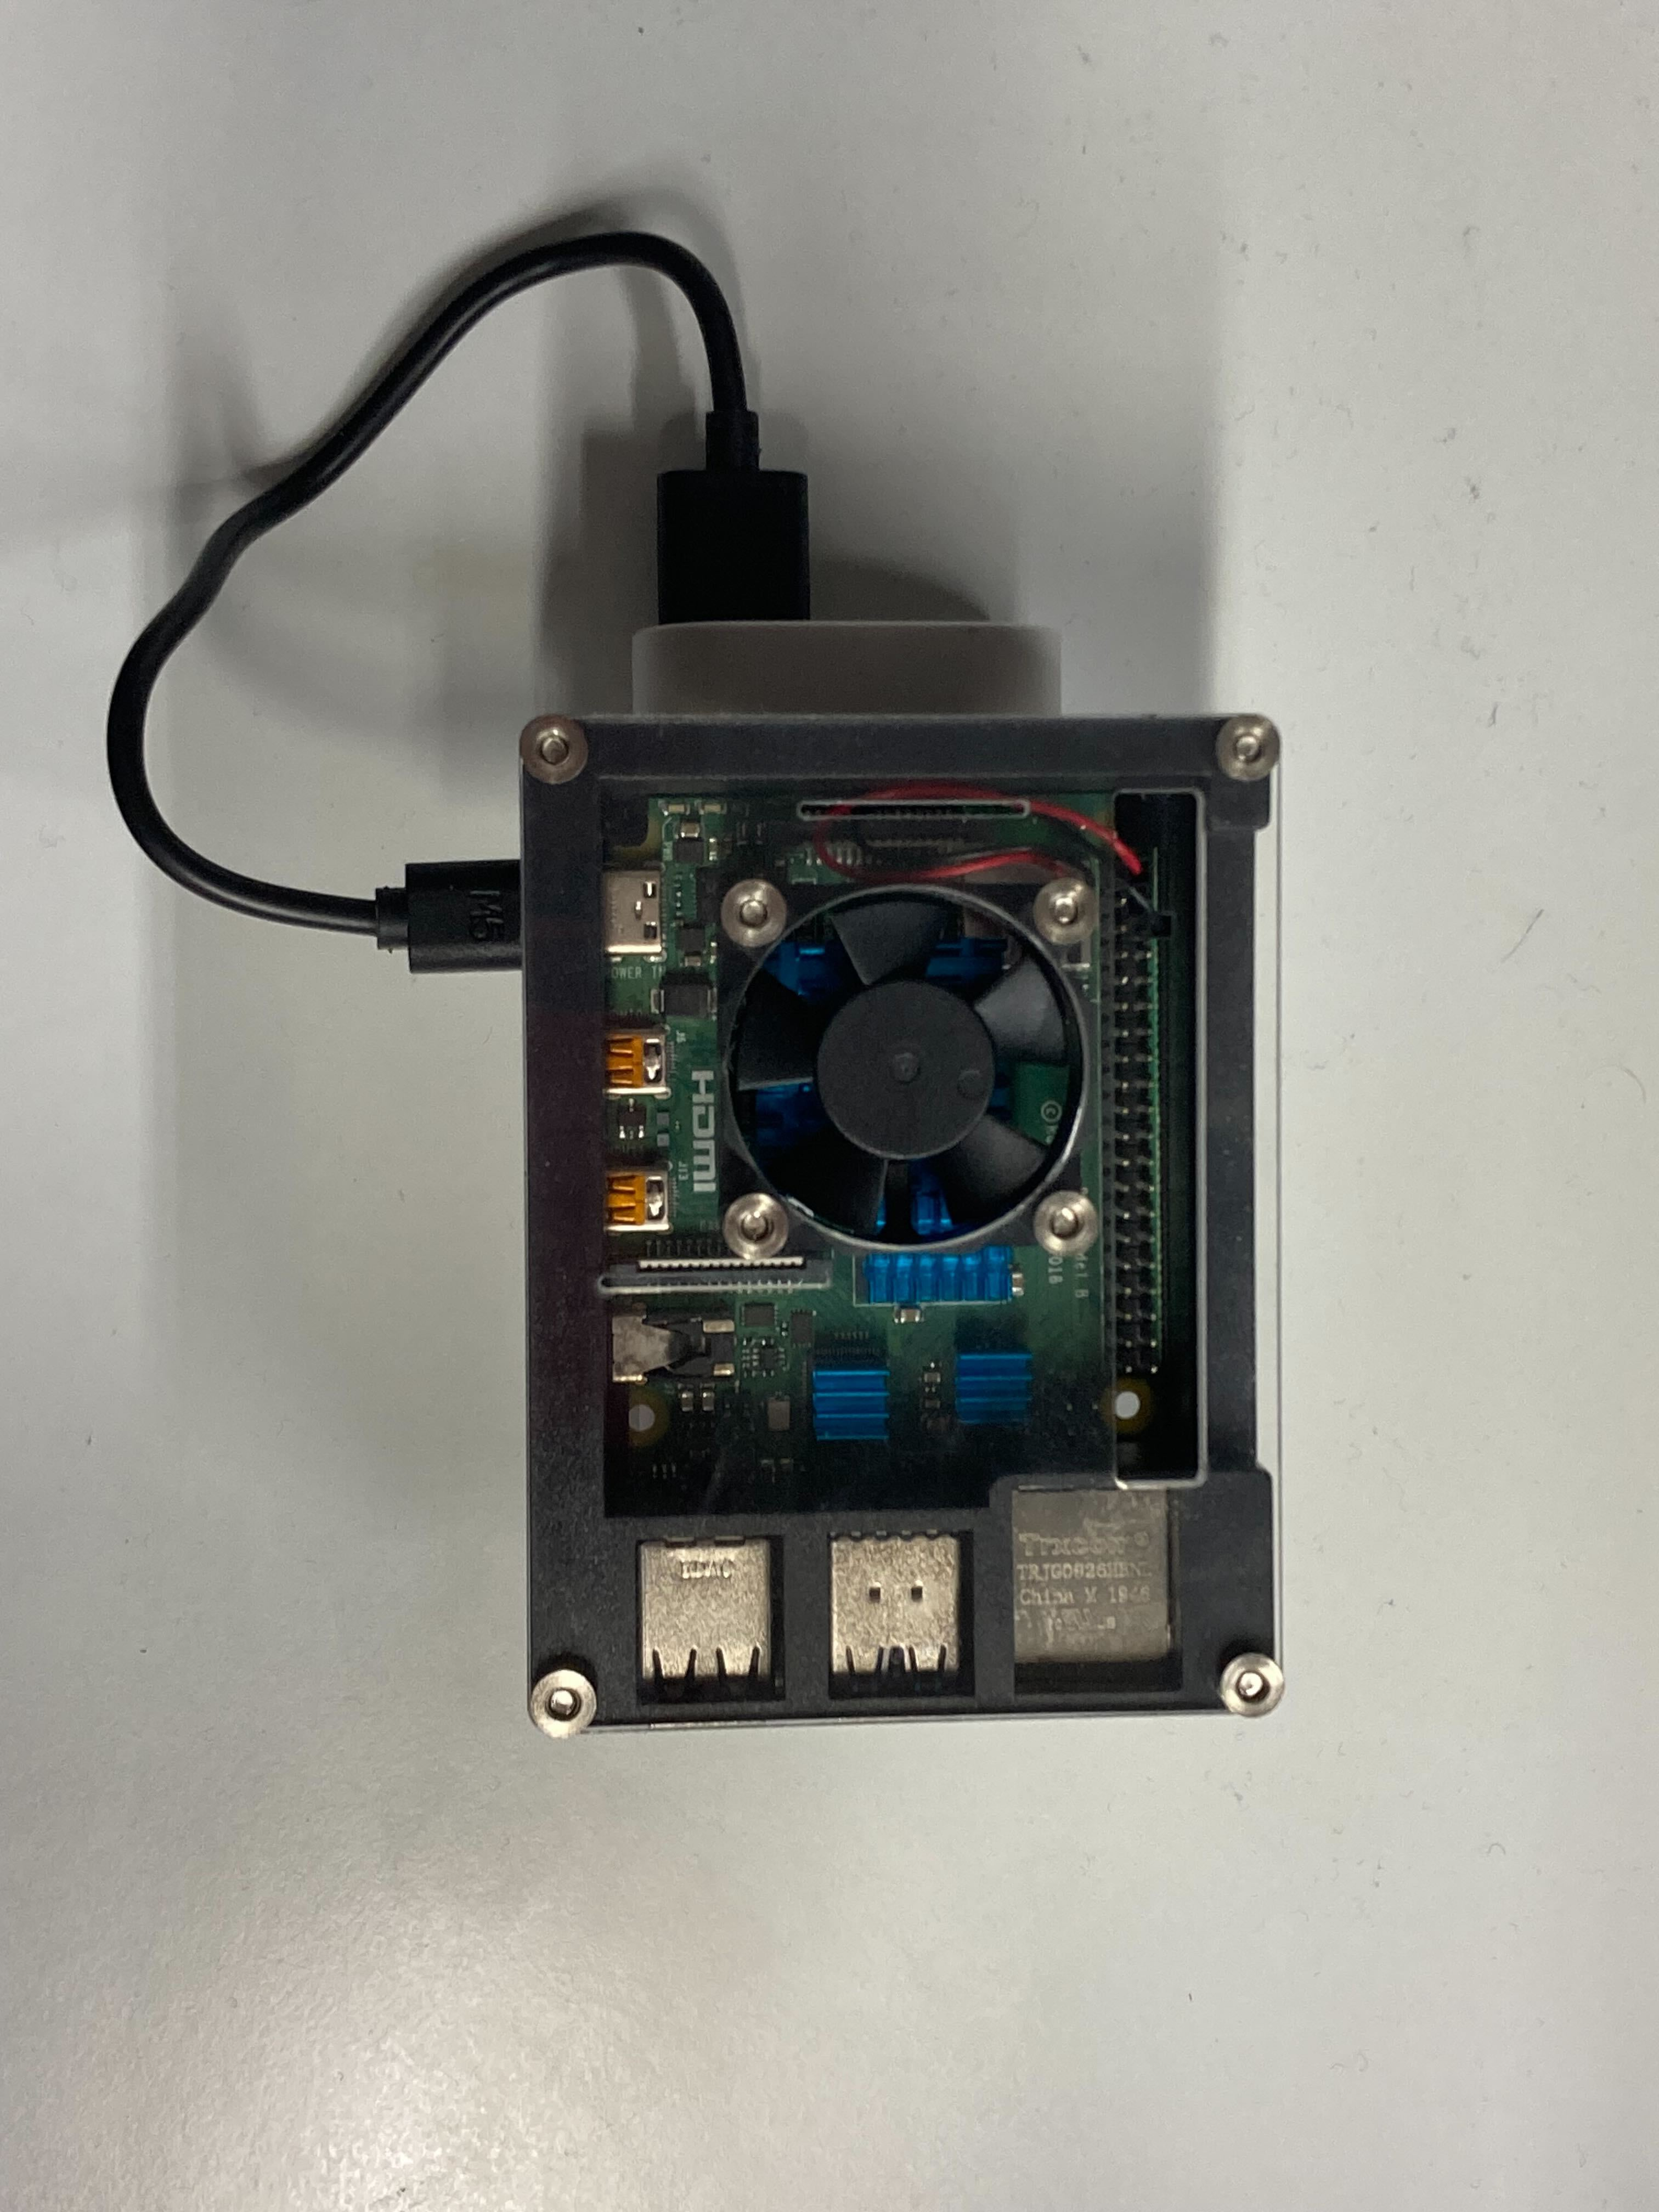
\includegraphics[scale=0.07]{./images/raspi.jpg}
  \centering
  \caption{設置したRaspberry Pi\label{raspi}}
\end{figure}

図\ref{raspi_place}に学生食堂の概略図とRaspberry Piの設置位置を示す.
基本的に壁などの空間を隔てるような障害物は存在せず,開けた空間となっており,そこに机や椅子が配置されている.
Raspberry Piは学生食堂1階と2階それぞれのフロアの中央に計2台配置する.
それぞれのRaspberry Piはお互いに異なるタイミングでスキャンを開始するため,
2台のRaspberry Piは同期していない.
Raspberry Piは1階と2階に配置するが,1階と2階は完全に別の空間ではなく,
スキャン範囲が重複していることに注意が必要である.
\begin{figure}[pt]
  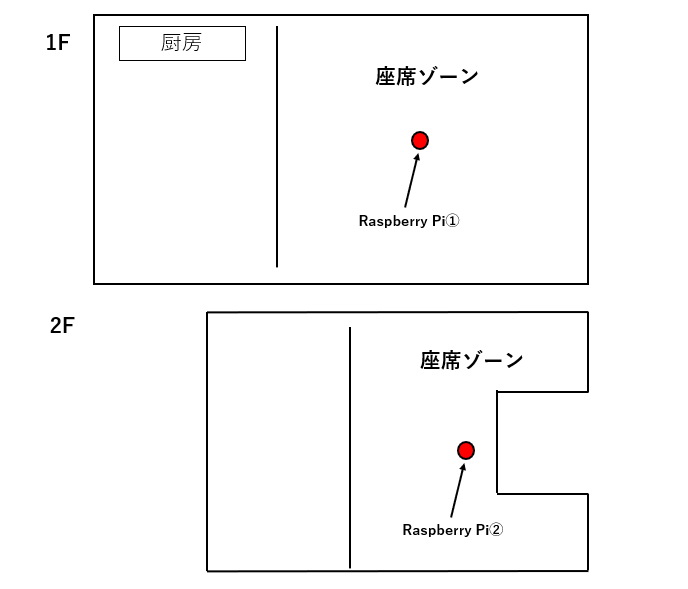
\includegraphics[scale=0.4]{./images/raspi_place.png}
  \centering
  \caption{学生食堂の概略図とRaspberry Piの設置位置\label{raspi_place}}
\end{figure}

\subsubsection*{食堂利用人数の計測}
学生食堂の利用人数は,愛媛大学生協の方に提供していただいた決済データの時間情報と,
利用者が食堂を退出する際に返却されるトレーの数を計測し,算出する.
トレーの数の計測は2人体制で行い,返却場所にカメラを設置する.
計測者間で大きくズレが発生している場合は,カメラを確認し,再度計測する.
決済データは1分間隔で提供されるため,BLEスキャンデータと同様に1分間隔で食堂利用人数を算出する.

\subsection*{3.2 特徴量抽出}
本プロジェクトでは,BLEスキャン情報から混雑度推定に有用な特徴量を抽出し,
モデルに入力することで混雑度を推定する.
基本的な特徴量は松田らの研究\cite{senkou}に基づき,表\ref{tbl:feastures}のように設計した.
unique\_num\_60\textsubscript{sec}\_$S$dbは,
RSSIの値$S$を閾値として,-60から-100まで,10ずつ変化させ,5つ特徴量を得る.
本プロジェクトでは,比較的大規模で開けた空間での混雑度推定を行う.
そのため障害物等による影響が少なく,RSSI値が比較的安定する.
そのためunique\_num\_60\textsubscript{sec}\_$S$dbのような特徴量を用いることで,
より安定した混雑度推定が可能になると考えられる.


\begin{table}[tb]
	\centering
	\caption{特徴量一覧}
	\label{tbl:feastures}
	\small
	\doublerulesep=0.3pt
    \begin{tabular}{l|p{5cm}} \hline\hline\hline
		特徴量名 & 内容 \\ \hline
		all\_num\_60\textsubscript{sec} & 過去 $T$ 秒間にスキャンされた,BD アドレスの総数\\ \hline
    unique\_num\_60\textsubscript{sec} & 過去 $T$ 秒間にスキャンされた,BD アドレスのユニーク数 \\ \hline
    unique\_ratio\_60\textsubscript{sec} & 過去 $T$ 秒間にスキャンされた,BD アドレスのうち,ユニークなデバイスの占める割合(ユニーク数 / 総数) \\ \hline
    unique\_num\_60\textsubscript{sec}\_$S$db & 過去 $T$ 秒間にスキャンされた,BD アドレスのうち,RSSI が閾値 Sdb より大きいもののユニーク数 \\ \hline\hline\hline
	\end{tabular}
\end{table}

\subsection*{3.3 混雑度推定モデル}
混雑度推定モデルは,BLEスキャン情報から抽出した特徴量を入力として,人数を出力するモデルである.
2.4節,2.5節で述べたモデルを用い,人数推定モデルを構築する.
詳しい学習の方法などは,A-4節で述べる.

\subsection*{3.4 評価指標}
本プロジェクトでモデルの性能評価に用いる指標について以下に述べる.

\subsubsection*{平均二乗誤差(Mean Squared Error, MSE)}
MSEは,予測値と実測値の差の二乗の平均を計算することにより,
モデルの誤差を定量化する指標である.数式で表すと,以下のようになる.
\begin{equation}
  \label{eq:mse}
  \mathrm{MSE} = \frac{1}{n} \sum_{i=1}^{n} (y_i - \hat{y}_i)^2
\end{equation}
ここで,$n$はサンプル数,$y_i$は実測値,$\hat{y}_i$は予測値である.
数値が低いほどモデルの性能が良いことを示す.
MSEは,誤差の二乗を取るため,外れ値が大きく影響する.

\subsubsection*{平均絶対誤差(Mean Absolute Error, MAE)}
MAEは,予測値と実測値の差の絶対値の平均を計算することにより,
モデルの誤差を定量化する指標である.数式で表すと,以下のようになる.
\begin{equation}
  \label{eq:mae}
  \mathrm{MAE} = \frac{1}{n} \sum_{i=1}^{n} |y_i - \hat{y}_i|
\end{equation}
ここで,$n$はサンプル数,$y_i$は実測値,$\hat{y}_i$は予測値である.
数値が低いほどモデルの性能が良いことを示す.
MAEは,MSEと比較して,外れ値の影響を受けにくい.

\subsubsection*{決定係数(Coefficient of Determination, $R^2$)}
決定係数は,予測値が実測値をどの程度説明できるかを示す指標である.  
数式で表すと,以下のようになる.
\begin{equation}
  \label{eq:r2}
  R^2 = 1 - \frac{\sum_{i=1}^{n} (y_i - \hat{y}_i)^2}{\sum_{i=1}^{n} (y_i - \bar{y})^2}
\end{equation}
ここで,$n$はサンプル数,$y_i$は実測値,$\hat{y}_i$は予測値,$\bar{y}$は実測値の平均である.
$R^2$の値は$0$から$1$の範囲を取り,$1$に近いほどモデルの性能が良いことを示す.
$R^2$は,モデルの説明力を示す指標であり,$0$に近い場合はモデルが実測値をほとんど説明できていないことを示す.